\chapter{Project Phases}
\label{chap:phases}

This chapter describes the project phases used in the planning and development of SitaWare Civilian.

Figure \ref{fig:project_phases} shows the six phases through which the system is to be developed. Furthermore, the figure contains the deliverables for the phase specific reviews. 

\begin{figure}[H]
\centering
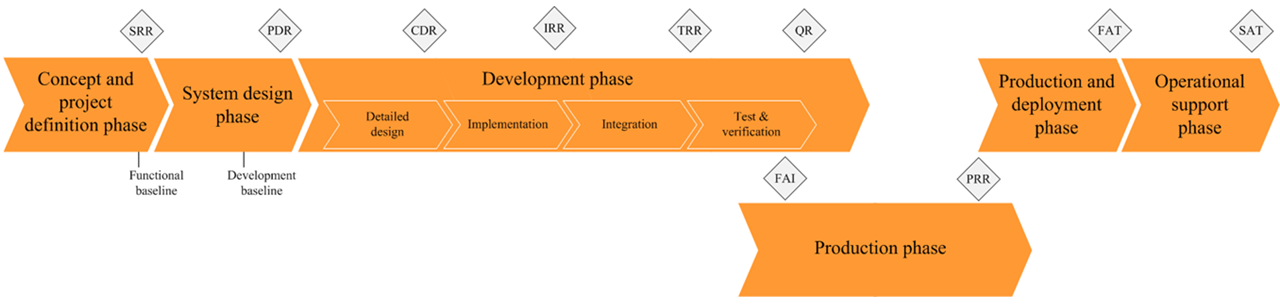
\includegraphics[width=0.95\textwidth]
{Billeder/project_phases/project_phases.PNG}
\caption{Project phases.}
\label{fig:project_phases}
\end{figure}


\paragraph{Concept and project definition phase}
This is the initial phase of the project and defines the problems and needs presented by the customer. By inspecting the needs, requirements to the system are identified. Furthermore, test methods for the defined requirements are specified. The phase ends with a system requirement review(SRR) between the development team and the customer. 

Deliverables:
\begin{enumerate}
\item[•] Time plan
\item[•] System Requirement Specification(SRS)
\item[•] Concept of Operations(CONOPS)
\item[•] Traceability matrix
\end{enumerate}


\paragraph{System design phase}
In this phase a plan for the conduct of the project is created. The plan covers what, by whom and when the different project elements are carried out. Furthermore, a preliminary design description is produced to close the gap between the requirements and the design phase, by clarifying the high-level design concept, which will implement the requirements in the SRS. The phase ends with a preliminary design review(PDR) between the development team and the customer. 

Deliverables:
\begin{enumerate}
\item[•] System Engineering Management Plan(SEMP)
\item[•] Preliminary Design Description(PDD)
\end{enumerate}


\paragraph{Development phase}
In this phase the actual product is designed, implemented, integrated and tested. The development phase consists of four subphases, each with their review: 
\begin{enumerate}
\item[•] Detailed design $\rightarrow$ Critical Design Review(CDR)
\item[•] Implementation $\rightarrow$ Integration Readiness Review(IRR)
\item[•] Integration $\rightarrow$ Test Readiness Review(TRR)
\item[•] Test and verification $\rightarrow$ Qualification Review(QR)
\end{enumerate}
All of the reviews are between the development team and the customer.

The following deliverables form the basis of the related reviews:
\begin{enumerate}
\item[•] Detailed Design Description(CDR)
\item[•] Minutes of SubContractor Meeting(CDR)
\item[•] Integration Plan(IRR)
\item[•] System Test Description(TRR)
\item[•] Test Results Description(QR)
\end{enumerate}


\paragraph{Production phase}
(This phase is not described.)

\paragraph{Production and deployment phase}
(This phase is not described.)

\paragraph{Operational support phase}
(This phase is not described.)